\documentclass[nols]{tufte-book}% or tufte-handout
\hypersetup{colorlinks}% uncomment this line if you prefer colored hyperlinks (e.g., for onscreen viewing)

%%
% Book metadata
\title{{M}arti{T}racks Manual\thanks{Thanks to Marti, gone but never forgotten.}}
\author[Daniel Rafael Miranda-Esquivel \& Susy Echeverr\'ia]{Daniel Rafael Miranda-Esquivel \& Susy Echeverr\'ia}
%\footnote{20072010}

\usepackage{natbib}

\usepackage{drme}


\bibliographystyle{./diver_distri}

\publisher{Published by the authors}


%%
% If they're installed, use Bergamo and Chantilly from www.fontsite.com.
% They're clones of Bembo and Gill Sans, respectively.
%\IfFileExists{bergamo.sty}{\usepackage[osf]{bergamo}}{}% Bembo
%\IfFileExists{chantill.sty}{\usepackage{chantill}}{}% Gill Sans

%\usepackage{microtype}

%%
% Just some sample text
\usepackage{lipsum}

%%
% For nicely typeset tabular material
\usepackage{booktabs}

%%
% For graphics / images
\usepackage{graphicx}
\setkeys{Gin}{width=\linewidth,totalheight=\textheight,keepaspectratio}
\graphicspath{{graphics/}}

% The fancyvrb package lets us customize the formatting of verbatim
% environments.  We use a slightly smaller font.
\usepackage{fancyvrb}
\fvset{fontsize=\normalsize}

%%
% Prints argument within hanging parentheses (i.e., parentheses that take
% up no horizontal space).  Useful in tabular environments.
\newcommand{\hangp}[1]{\makebox[0pt][r]{(}#1\makebox[0pt][l]{)}}

%%
% Prints an asterisk that takes up no horizontal space.
% Useful in tabular environments.
\newcommand{\hangstar}{\makebox[0pt][l]{*}}

%%
% Prints a trailing space in a smart way.

%
\usepackage{xspace}

%%
% Some shortcuts for Tufte's book titles.  The lowercase commands will
% produce the initials of the book title in italics.  The all-caps commands
% will print out the full title of the book in italics.
\newcommand{\vdqi}{\textit{VDQI}\xspace}
\newcommand{\ei}{\textit{EI}\xspace}
\newcommand{\ve}{\textit{VE}\xspace}
\newcommand{\be}{\textit{BE}\xspace}
\newcommand{\VDQI}{\textit{The Visual Display of Quantitative Information}\xspace}
\newcommand{\EI}{\textit{Envisioning Information}\xspace}
\newcommand{\VE}{\textit{Visual Explanations}\xspace}
\newcommand{\BE}{\textit{Beautiful Evidence}\xspace}

\newcommand{\TL}{Tufte-\LaTeX\xspace}

% Prints the month name (e.g., January) and the year (e.g., 2008)
\newcommand{\monthyear}{%
  \ifcase\month\or January\or February\or March\or April\or May\or June\or
  July\or August\or September\or October\or November\or
  December\fi\space\number\year
}


% Prints an epigraph and speaker in sans serif, all-caps type.
\newcommand{\openepigraph}[2]{%
  %\sffamily\fontsize{14}{16}\selectfont
  \begin{fullwidth}
  \sffamily\large
  \begin{doublespace}
  \noindent\allcaps{#1}\\% epigraph
  \noindent\allcaps{#2}% author
  \end{doublespace}
  \end{fullwidth}
}

% Inserts a blank page
\newcommand{\blankpage}{\newpage\hbox{}\thispagestyle{empty}\newpage}

\usepackage{units}

% Typesets the font size, leading, and measure in the form of 10/12x26 pc.
\newcommand{\measure}[3]{#1/#2$\times$\unit[#3]{pc}}

% Macros for typesetting the documentation
\newcommand{\hlred}[1]{\textcolor{Maroon}{#1}}% prints in red
\newcommand{\hangleft}[1]{\makebox[0pt][r]{#1}}
\newcommand{\hairsp}{\hspace{1pt}}% hair space
\newcommand{\hquad}{\hskip0.5em\relax}% half quad space
\newcommand{\TODO}{\textcolor{red}{\bf TODO!}\xspace}
\newcommand{\ie}{\textit{i.\hairsp{}e.}\xspace}
\newcommand{\eg}{\textit{e.\hairsp{}g.}\xspace}
\newcommand{\na}{\quad--}% used in tables for N/A cells
\providecommand{\XeLaTeX}{X\lower.5ex\hbox{\kern-0.15em\reflectbox{E}}\kern-0.1em\LaTeX}
\newcommand{\tXeLaTeX}{\XeLaTeX\index{XeLaTeX@\protect\XeLaTeX}}
% \index{\texttt{\textbackslash xyz}@\hangleft{\texttt{\textbackslash}}\texttt{xyz}}
\newcommand{\tuftebs}{\symbol{'134}}% a backslash in tt type in OT1/T1
\newcommand{\doccmdnoindex}[2][]{\texttt{\tuftebs#2}}% command name -- adds backslash automatically (and doesn't add cmd to the index)
\newcommand{\doccmddef}[2][]{%
  \hlred{\texttt{\tuftebs#2}}\label{cmd:#2}%
  \ifthenelse{\isempty{#1}}%
    {% add the command to the index
      \index{#2 command@\protect\hangleft{\texttt{\tuftebs}}\texttt{#2}}% command name
    }%
    {% add the command and package to the index
      \index{#2 command@\protect\hangleft{\texttt{\tuftebs}}\texttt{#2} (\texttt{#1} package)}% command name
      \index{#1 package@\texttt{#1} package}\index{packages!#1@\texttt{#1}}% package name
    }%
}% command name -- adds backslash automatically
\newcommand{\doccmd}[2][]{%
  \texttt{\tuftebs#2}%
  \ifthenelse{\isempty{#1}}%
    {% add the command to the index
      \index{#2 command@\protect\hangleft{\texttt{\tuftebs}}\texttt{#2}}% command name
    }%
    {% add the command and package to the index
      \index{#2 command@\protect\hangleft{\texttt{\tuftebs}}\texttt{#2} (\texttt{#1} package)}% command name
      \index{#1 package@\texttt{#1} package}\index{packages!#1@\texttt{#1}}% package name
    }%
}% command name -- adds backslash automatically
\newcommand{\docopt}[1]{\ensuremath{\langle}\textrm{\textit{#1}}\ensuremath{\rangle}}% optional command argument
\newcommand{\docarg}[1]{\textrm{\textit{#1}}}% (required) command argument
\newenvironment{docspec}{\begin{quotation}\ttfamily\parskip0pt\parindent0pt\ignorespaces}{\end{quotation}}% command specification environment
\newcommand{\docenv}[1]{\texttt{#1}\index{#1 environment@\texttt{#1} environment}\index{environments!#1@\texttt{#1}}}% environment name
\newcommand{\docenvdef}[1]{\hlred{\texttt{#1}}\label{env:#1}\index{#1 environment@\texttt{#1} environment}\index{environments!#1@\texttt{#1}}}% environment name
\newcommand{\docpkg}[1]{\texttt{#1}\index{#1 package@\texttt{#1} package}\index{packages!#1@\texttt{#1}}}% package name
\newcommand{\doccls}[1]{\texttt{#1}}% document class name
\newcommand{\docclsopt}[1]{\texttt{#1}\index{#1 class option@\texttt{#1} class option}\index{class options!#1@\texttt{#1}}}% document class option name
\newcommand{\docclsoptdef}[1]{\hlred{\texttt{#1}}\label{clsopt:#1}\index{#1 class option@\texttt{#1} class option}\index{class options!#1@\texttt{#1}}}% document class option name defined
\newcommand{\docmsg}[2]{\bigskip\begin{fullwidth}\noindent\ttfamily#1\end{fullwidth}\medskip\par\noindent#2}
\newcommand{\docfilehook}[2]{\texttt{#1}\index{file hooks!#2}\index{#1@\texttt{#1}}}
\newcommand{\doccounter}[1]{\texttt{#1}\index{#1 counter@\texttt{#1} counter}}


\linespread{1.4}


% Generates the index
\usepackage{makeidx}

\makeindex
% 

\begin{document}



% 
% 


% \begin{figure} %[!ht]
% \begin{center}
% % \includegraphics[scale=0.15]{./logo0-marti.jpg}
% \includegraphics{./graphics/logo0-marti.jpg}
% 
% \end{center}
% \end{figure}
% 
% Front matter
\frontmatter

% r.1 blank page
%\blankpage

% v.2 epigraphs
%\newpage\thispagestyle{empty}


% r.3 full title page
\maketitle


% v.4 copyright page
\newpage
\begin{fullwidth}
~\vfill
\thispagestyle{empty}
\setlength{\parindent}{0pt}
\setlength{\parskip}{\baselineskip}
Copyright \copyright\ \the\year\ \thanklessauthor


%\par\smallcaps{Published by \thanklesspublisher}

\par\smallcaps{Based on  \TL, please refer to  \url{tufte-latex.googlecode.com} for further information}

\par Licensed under the Apache License, Version 2.0 (the ``License''); you may not
use this file except in compliance with the License. You may obtain a copy
of the License at \url{http://www.apache.org/licenses/LICENSE-2.0}. Unless
required by applicable law or agreed to in writing, software distributed
under the License is distributed on an \smallcaps{``AS IS'' BASIS, WITHOUT
WARRANTIES OR CONDITIONS OF ANY KIND}, either express or implied. See the
License for the specific language governing permissions and limitations
under the License.\index{license}

\end{fullwidth}

%\par\textit{First printing, \monthyear}

\vfill
\openepigraph{Life and Earth have evolved together}{Leon Croizat}
\openepigraph{Analyses and Software have to evolve together}{The authors}

% r.5 contents
\tableofcontents

\listoffigures

\listoftables

% r.7 dedication
\cleardoublepage
~\vfill
\begin{doublespace}
\noindent\fontsize{18}{22}\selectfont\itshape
\nohyphenation
Dedicated to those who appreciate good Biogeography and love dogs.
\end{doublespace}
%\vfill

\chapter{Forewords}

This manual is intended to be a clear and comprensive 
introduction to Panbiogeography and geometric track analyses, using the program \MT. 
The book is divided into four main chapters and some appendices.
First chapter is a general introduction to Panbiogeography and related terms, second chapter presents
\MT' algorithm while third chapter is devoted to commands used. The fourth and final chapter presents
some theorethical and empirical data and its analyses to explore \MT options.


\vspace{-7\baselineskip}\footnotetext{\url{http://ciencias.uis.edu.co/labsist/pantrack}}
\vspace{7\baselineskip}


The program was developed using FreePascal, as Pascal is an intuitive and easy to handdle language for programming, 
the debate is open to consider whether C/C++ or Phython/Perl/Java are more suitable languages for this kind of problem. As a free
software project, feel free to criticize the code or the algorithm, and if you improve it, we will be more than delighted and thankful. 


\vspace{-7\baselineskip}\footnotetext{\url{http://www.freepascal.org}}
\vspace{7\baselineskip}

This manual has been developed using \TL, maybe (in our humble opinion), the best environment to write a book or a handout.



We are grateful to many people, .....

We are open to new ideas or suggestions to improve our analyses, the program, and this manual itself. 

\vspace{-7\baselineskip}\footnotetext{\url{http://code.google.com/p/tufte-latex}}
\vspace{7\baselineskip}

\mainmatter

% r.9 introduction
%\cleardoublepage

\chapter{Introduction}
\label{ch:panbio}


\section{Panbiogeography}

Panbiogeography is a unique and very useful approach to capture any
distributional pattern/structure in studies that use geographical data. Mapping
biogeographic tracks is a cost efficient way to reduce the initial complexity
that we find in the data sets \citep{Craw1989a}, as Croizat's tracks analysis
\citep{croizat1952, Croizat1958} provides a conceptual
framework for understanding the biogeographic structure and the relationships of
areas.

\index{Croizat:books}
Panbiogeography was developed by Croizat in his books, ''Manual of
phytogeography''\citep{croizat1952}, ''Panbiogeography''\citep{Croizat1958} and
''Space, Time, Form: The Biological Synthesis''\citep{Croizat1964}.
Panbiogeography was inspired by Croizat's idea of connecting two essential
elements in evolution: Space and Time: Earth and Life evolve together, which
means that biotas evolve together with the geographic barriers
\citep{MorroneCrisci1995, Morrone2000}.

Croizat's panbiogeography constituted a unique critique to Darwin's biogeography
ideas about natural selection, means of dispersal and geographic distribution
\citep{Craw1987}. This approach challenged the idea that means of
dispersal are the principal factors responsible for the evolution of the
distribution \citep{Craw1989b, Crawetal1999}.

Panbiogeography assumes that taxa distribution evolves through two stages:
mobilism and immobilism. The interaction of these two states is called vicariant
form-making model. Within the mobilism stage, an ancestor taxon expands to
establish on new territory through its means of dispersal (''means of
survival'') when the geographic and climatic factors are favorable. Later, when
the range geographic is established (immobilism) the appearance of barriers
allows the isolation and differentiation of taxa (vicariant form-making)
\citep{Grehan1988a, Michaux1989,  Crawetal1999, CrisciMorrone1992a}.

Panbiogeography has been considered an independent research program because is
the only approach that focuses on the spatial or geographical sector as a
fundamental pre-condition to any analysis of the patterns and processes of
evolutionary change \citep{Crawetal1999, Grehan1994, Grehan2001a}.

The assumptions that make the Panbiogeography different from other historical
biogeography approaches are \citep[][:19]{Crawetal1999}:
\index{Panbiogeography:assumptions}
''1. Distribution patterns constitute an empirical databases for biogeographical
analysis.

2. Distribution patterns provide information about where, when, and how animals
ans plants evolve;

3. The spatial and temporal component of these distribution patterns can be
graphically represented;

4. Testable hypothesis about historical relationship between the evolution of
distributions and Earth history can be derived from geographic correlations
between distribution graphs as geological/geomorphic features.''




\subsection{Track analysis}


Panbiogeography as a biogeographic method is called track analysis. There
are four principal concepts within this method: track, node, main massing, and
baseline \citep{CrisciMorrone1992a, Crawetal1999, Grehan2001a,
Espinosaetal2002}.
\index{Track analysis}
\index{Track analysis:individual tracks}

Individual tracks are the basic units of panbiogeography. These are lines drawn
on a map that connect different localities or distribution points of a
particular taxon or group of taxa, so that the sum of the segment lengths that
connect all the distribution points is the smallest possible. In the graph
theory words, the individual track is a minimum spanning tree
\citep{Crawetal1999, Morrone2004c, Page1987}
\index{Track analysis:generalized tracks}

Generalized tracks or standard tracks are called repetitive patterns because
summarized distributions of diverse individual taxa \citep{Michaux1989}. These
are lines on a map resulting from the superimposition of the individual tracks.
Generalized tracks are interpreted as distributional patterns of ancestral biota
that had been fragmented by tectonic and climatic events \citep{Craw1988}. These
panbiogeographic element is considered conjectures on a common biogeography
history or primary biogeography homology sensu  \citet{Morrone2001a}, which means
that analyzed taxa are spatiotemporally integrated in a biota \citep{Craw1983a,
Morrone2001a, Morrone2004c}.
\index{Track analysis:nodes}

Nodes are areas or localities where two or more generalized tracks are
overlapped. These are complex areas or tectonic and biotic convergence zones
\citep{Craw1988b, CrisciMorrone1992a, Morrone2004c, Page1987}. The nodes are
considered priority areas for conservation or sites of biological endemism
because represented localities of high diversity, distribution boundaries,
disjunction, incongruence and recombination, specimens that are difficult to
identify and unusual hybrids \citep{Crawetal1999, MorroneEspinosa1998,
Grehan1993}.


The Panbiogeographic method involves basically main three steps
\citep{Morrone2004c}: Firstly, construction of two or more taxon individual
tracks (minimum spanning tree from distributional localities). Secondly,
delimitation of generalized tracks through geographic congruence between
individual tracks. Finally, determination of nodes within the intersection areas
between generalized tracks.

There are different approaches within panbiogeographic method. Croizat`s manual
reconstruction \citep{Croizat1958, Croizat1964}, Page's Spanning graphs
\citep{Page1987}, Craw's Track compatibility \citep{Craw1989a} and PAE
(''Parsimony Analysis of Endemicity'') \citep{Rosen1984, Crawetal1999,
Luna-vegaetal2000, MorroneMarquez2001}
\index{PAE}

\index{Track analysis:manual reconstruction}


\subsection{Croizat's manual reconstruction}

Croizat's manual reconstruction is done by drawing on a map taxon's individual
tracks and then overlapping them to determinate generalized tracks. Basically
the method consists of the following steps \citep{Morrone2004c}:

1. Connect the disjunct areas of distribution by lines forming individual tracks,

2. The individual tracks are oriented using baselines,

3. Overlap individual tracks to determinate generalized tracks,

4. Recognize the nodes where two or more generalized tracks are intersected,

5. Indicate on a map the generalized tracks,baselines and nodes.


\subsection{Page's Spanning graphs}

Page's Spanning graphs was the first attempt to quantify the panbiogeographic
analysis using graph theory. Its main methodological steps are \citep{Page1987}:
\index{Page's Spanning graphs}

1. connect the disjunct areas of distribution through a MST (Minimum Spanning
Trees) forming an individual track for each species,

2. Construct incidence and connectivity
matrices for individual tracks to recognized shared elements and track
congruence,

3. Construct a connectivity matrix for all tracks together to search
circuits that indicate incongruence tracks,

4. Indicate on a map the generalized
tracks, baselines and nodes.

\subsection{Craw's tracks compatibility analysis}
\index{Craw's tracks compatibility analysis}

Craw's tracks compatibility analysis \citep{Craw1989a} involves finding the
largest clique of compatible tracks through a locality/distribution per track
matrix \citep{Crawetal1999}. In general, its algorithm involves the following
steps \citep{Craw1989a, Grehan2001c, Morrone2004c}:

1. Construct individual tracks for different taxa from distribution localities using a MST,

2. Generate an areas matrix for individual tracks where the presence of the areas is
represented by ''1'' and absence by ''0''.

3. Find the largest clique for compatible individual tracks which is considered the generalized track.

4. Evaluate statistically the generalized track,

5. Indicate on a map the
generalized tracks, baselines, and nodes.


\subsection{Parsimony Analysis of Endemicity}

\index{PAE:algorithm}

PAE (''Parsimony Analysis of Endemicity'') has been considered a
panbiogeographic method \citep{Crawetal1999, Luna-vegaetal2000,
MorroneMarquez2001, Morrone2004c}. Its algorithm includes the following steps
\citep {Morrone2004c}:

1. Construct individual tracks for different taxa from distribution localities using a MST,

2. Generate an areas matrix for individual tracks where the presence of a species is represented by ''1'' and the absence by ''0''. Within this step, an extra area is added with ''0'' (all species absence) for polarized areas cladogram,

3. Analize the matrix using a parsimony algorithm. Each clade formed by at least two individual tracks is considered a generalized track,

4. ''Disconnect'' or delete the species that support the different clades and reanalyze the matrix to search clades that are supported by other taxa,

5. Indicate on a map the generalized tracks, baselines and nodes.

Since \citet{Croizat1958, Croizat1964} presented his panbiogeographic method,
the above mentioned quantitative techniques had been proposed, Page's graph
theory method \citep{Page1987},
Henderson's analysis \citep{Henderson1989}, which is similar to Page's analysis,
and Craw's compatibility track analysis \citep{Craw1989a}. These techniques have
emerged taking
into account Croizat's framework for analysis: individual tracks congruence to
define generalized tracks \citep{Page1987, Henderson1989, Craw1989b}.
\citet{Page1987} suggested a quantitative approach using graph theory by
incidence and connectivity matrices, but this method has not been applied to
real data, perhaps because of its difficult calculation and computational
complexity. \citet{Craw1989a} proposed the compatibility track analysis based on
distributional compatibility which is analogous with Meacham's character
compatibility approach \citep{Meacham1984} to phylogenetic systematics
\citep{Crawetal1999}. Within the latter method, two or more individual tracks
are considered compatible if either one is included within or replicated by the
other. \citet{MorroneCrisci1995} claimed that the compatibility in
Panbiogeography is used in a restricted way depending on the method.
''Non-overlapping tracks'' are incompatible according to compatibility track
analysis and should be compatible in Croizat's track analysis by geographic
proximity.

Within the quantitative techniques proposed in the history of the
panbiogeography \citep{Page1987, Craw1989a, Henderson1989}, only
Craw`s compatibility tracks analysis has been implemented and now part of the
algorithm, the minimal spanning tree, has been automated in the software
package ''Croizat'' \citep{Cavalcanti2009b}.

Grid analysis such as PAE (Parsimony Analysis of Endemicity) has been
considered a panbiogeographic approach \citep{Crawetal1999, Luna-vegaetal2000,
MorroneMarquez2001, Morrone2004c}, but some authors do not consider it a
historical biogeography method \citep{Humphries2000, Garcia-Barros2002}.
Although this method has been widely used \citep{Luna-vegaetal2000,
MorroneMarquez2001, Huidobroetal2006, Mihocetal2006, Espinosa-Perezetal2009,
Contreras-Medinaetal2007}, its implementation to the panbiogeographic analysis
was secondary. Its direct objective is the analysis of endemism and its relation
to the track analysis sensu Croizat could become ambiguous.

Despite of these methods, Croizat's manual reconstruction has been the most used
in panbiogeographic studies because its simplicity and the alleged direct
connection to Croizat's panbiogeographic concept. Nevertheless, the debate about
the reliability of the manual reconstruction is still
valid. The method turns to be ambiguous and generates subjective results with
large data set due to overcrowded points \citep{Franco-Rosselli2001, Liria2008}.



\section{Suggested literature}

\begin{itemize}
\item \citet{Crawetal1999} is a good summary of theories and methods, while the
empirical approach could be flawed.

\item \citet{Crisci2001} is an historical account of biogeography, and is
ilustrative of the so called forces that shaped present biogeographic thought.
\end{itemize}




\chapter{PanTrack, the program}


\section*{Definitions}

% %
% %CADA activida debeestar ligada
% a un deseo potencial
% 
% imnPGT you cando X and Y. To do X 
% 


\MT algorithm has been presented in our paper (cite), therefore we suggest you to read the paper first.


The program tracks MST or segments, therefore you can conduct your analysis in either of those two ways.

\vspace{-7\baselineskip}\footnotetext{If your are not familiar with graph theory you might find theses links useful: 

 \url{http://en.wikipedia.org/wiki/Minimum_spanning_tree}

 \url{http://en.wikipedia.org/wiki/Glossary_of_graph_theory}}
\vspace{7\baselineskip}




\section*{The program and its calculations}


If you use MST, the species' MST will be compared to all species MST, comparing each segment but outputing the answer by species, so you can expect at most nsp posible tracks, where nsp is the number of initial species.
	

\vspace{-7\baselineskip}\footnotetext{nsp = number of species}
\vspace{7\baselineskip}

If you use segments each segment will be compared to all species MST, comparing each segment and outputing the answer by segments/points, so you can expect at most nsegs, where nseg is
	
	sum MST(i)
		j=1 -$>$ nsp
		i=number of segments MST(j)
		    
		
As all segments or MST are not congruent, the real number of answers lies in a number smaller than those.



\subsection*{\MT files. General information}


The program uses two input files,



1. -the input file with the distributional data. (Only the input file is mandatory).
	
	
2. -the parameters/orders file with the values for parameters and the commands to be executed in bash 
	

	
and creates a kml output file


\subsection*{\MT input file}

\MT accepts as an input, a text file comprised of three columns,
	
	labels   lat   long
	

separated by tabs or spaces but not commas (,), most spreadsheet and sig programs can output shuch text files, or you can use awk/bash to reshape them. 


\label{valid_data_set}
\index{valid input data set}

\vspace{-7\baselineskip}\footnotetext{a valid data set = test0.dat

\begin{center} 
\begin{tabular}{lll}
sp1 & 1 & 9\\
sp1 & 3 & 11\\
sp1 & 6 & 12\\
sp2 & 1 & 9\\
sp2 & 1 & 10\\
sp2 & 3 & 10\\
sp2 & 4 & 11\\
sp2 & 5 & 12\\
sp2 & 6 & 12\\
sp3 & 4 & 13\\
sp3 & 5 & 11\\
sp3 & 8 & 8\\
sp4 & 4 & 12\\
sp4 & 6 & 11\\
sp4 & 7 & 8\\
sp5 & 8 & 8\\
sp5 & 7 & 6\\
sp5 & 8 & 2\\
sp6 & 8 & 8\\
sp6 & 7 & 5\\
sp6 & 8 & 3
\end{tabular}
% \caption{data from test0.dat}
 

\end{center}

}
\vspace{7\baselineskip}
	
As an example we include 

		-a bash+awk command file that converts a comma delimitated file in a \mt inputfile (csv2pt.sh)

		-a bash+awk command file that converts a GlobalMapper output in a \mt inputfile (gm2pt.sh)


\vspace{-7\baselineskip}\footnotetext{note: if your label field includes inner tabs/spaces, these will be considered as field separator therefore are NOT allowed, you can replace 
	such character by an underscore or delete them all (\mt converts the dash to underscore)}
\vspace{7\baselineskip}
		 
	 

\vspace{-7\baselineskip}\footnotetext{A common mistake is different labels for the same species, although \mt
	is not case sensitive, it is (quite) sensitive to mispellings therefore
	\cmd{Simulium} and \cmd{simulium} are the same, while \cmd{Simuliium}, \cmd{Simuliiun} or \cmd{Simuliun} are not.}
\vspace{7\baselineskip}
	
	
\subsection*{\mt output file}

\MT writes kml files, with or without the initial tracks. With all the analyses made before closing, in the form of tracks or points. The output is easily readable using google-earth or gis programs as QGIS. As some programs may or may not read the output, we only keep compatibility with google-earth/QGIS. If your beloved gis program does not read the output, please consider read it with google-earth.




\section{Download the program and a data set}
\index{download the program}
\label{download}

You must download a binary for your plataform of choice, from  \url{http://tux.uis.edu.co/labsist/martitracks} or \url{http://code.google.com/p/martitracks/}


Binaries are provided for Linux 64, Win 32 and 64


and the data sets at \url{http://tux.uis.edu.co/labsist/martitracks/data-example.zip}


\vspace{-7\baselineskip}\footnotetext{For linux version, you might need to convert the file \mt-xx to an execute file by typing in a command-line window:

 \framebox[2in][l] {\prompt \cmd{chmod +x \mt}}}
\vspace{7\baselineskip}


\section{Command modes}
\index{command modes}

\MT has two uses-interfaces: 1. A text user interface, and 2. a command-line interface. 


in the text user interface (TUI), the user can choice among different options including: changes of parameters for analysis, track a pair, groups or the whole data, find the index of congruence (IC) between pairs of tracks, or among sevaral tracks. print kml file, etc.
The command line interface was created for search strategies previously defined. The input file, output file and parameters files must be defined.

\vspace{-7\baselineskip}\footnotetext{\url{http://en.wikipedia.org/wiki/Text_user_interface\#TUI_under_Unix-like_systems}}
\vspace{7\baselineskip}

\subsection{Text user interface}

\index{tui:text user interface}

\label{openprogram}

You can use the text interface by simply typing at the promt: 

\framebox[2in][l] {\prompt \cmd{ ./{\mt} }}

for Linux, and 

\framebox[2in][l] {\prompt \cmd{ {\mt-winXX.exe} }}

for Windows in a command-line window 


or by clicking on the \MT icon (win. only).

 
\vspace{-7\baselineskip}\footnotetext{
TUI typography: commands will be  \tui{c}ut, to indicate that the instruction is cut and the letter to be pressed is c]}
\vspace{7\baselineskip}


\textbf{1. Enter the input name}: As soon as you open \mt, it asks for the input file name:

\begin{center}
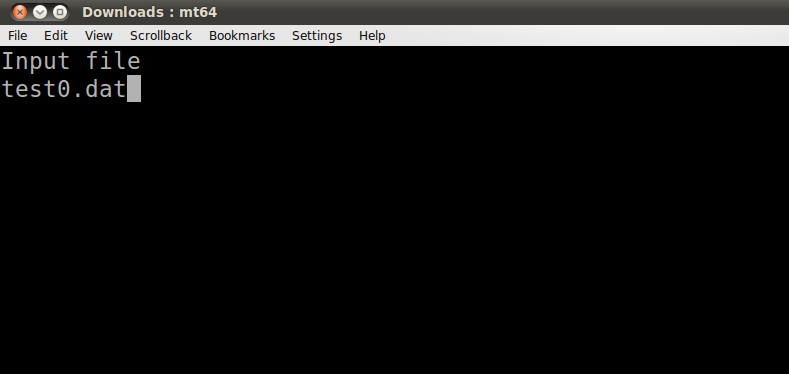
\includegraphics[scale=0.4]{./graphics/input-file.png}
 % input-file.png: 789x374 pixel, 72dpi, 27.83x13.19 cm, bb=0 0 789 374
\end{center}

\textbf{2. Set up the analysis:} Once you specified the input name, a list of commands help the users to set up the analysis.

\begin{center}
 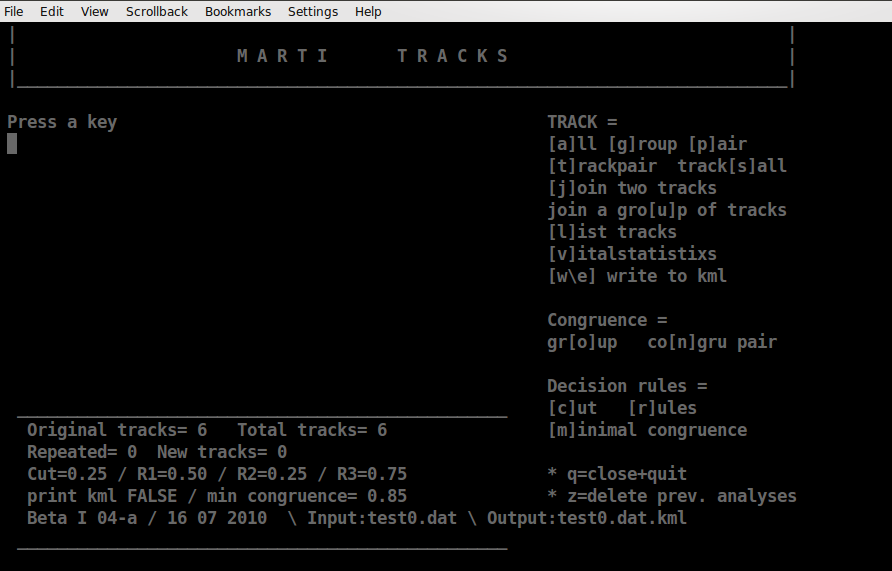
\includegraphics[scale=0.4]{./graphics/text-interface.png}
 % text-interface.png: 1237x678 pixel, 72dpi, 43.63x23.92 cm, bb=0 0 1237 678
\end{center}


Then we must define the values of the parameters, to be used in this analysis. 

There are five parameters: \tui{c}ut value, 

three \tui{r}ules of decision,  and the value for \tui{m}inimal congruence.

And we are ready to conduct our analysis. As we might have similar initial MSTs, we need to joint those MST that are the same according to the minimum value of \tui{m}inimal congruence fixed. We must press \tui{u}, to join the gro\tui{u}p. The program will ask thenumber of the initial and final track to be joint. Now we must use  \tui{a}ll, to find the congruent segments and define  the generalized tracks or distributional patterns of species. 

Finally, we need to eliminate those redundant generalized tracks, typing again \tui{u}, but joint from the track number 7  to the track 9, because first six tracks are individual tracks.

If, we want to write our results  in a kml file, we must type \tui{k} and \tui{+} to activate the output to the  kml file. The kml info must change from FALSE to TRUE. Then, we will use \tui{w} if we want to write the whole information of the analysis including: individual tracks, and generalized tracks, or we can type \tui{e} to write only the generalized tracks into the kml file.


For the command-line user interface we need to specified: the input file, output file, and parameters file.


\framebox[4.4in][l] {\prompt \cmd{ ./{\mt}-64 <input file> <output file> <parameters file>}}





\chapter{Worked examples}



% \begin{figure*}[p]
% \fbox{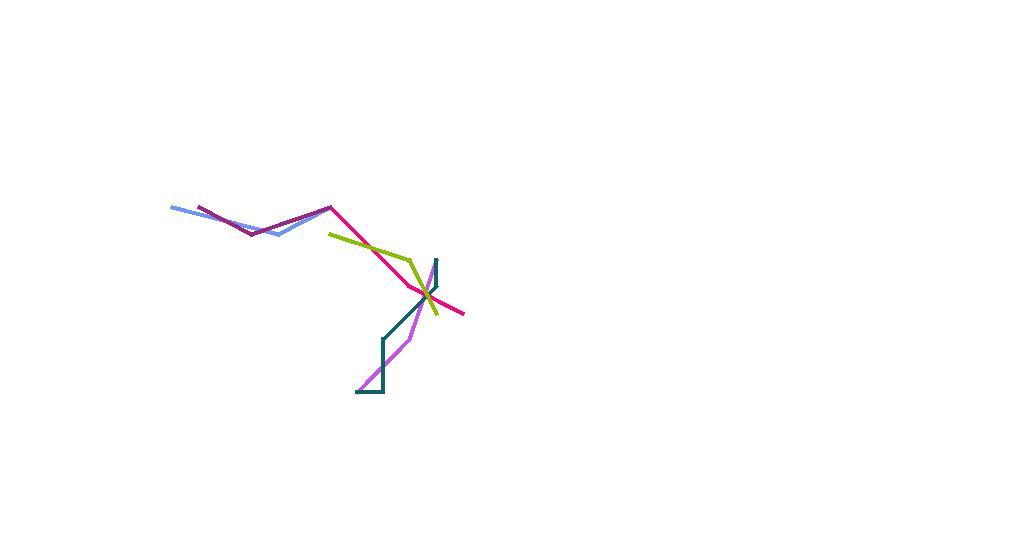
\includegraphics[width=0.85\linewidth]{1-6.png}}
% \end{figure*}
% 
% 
% \begin{figure*}[p]
% \fbox{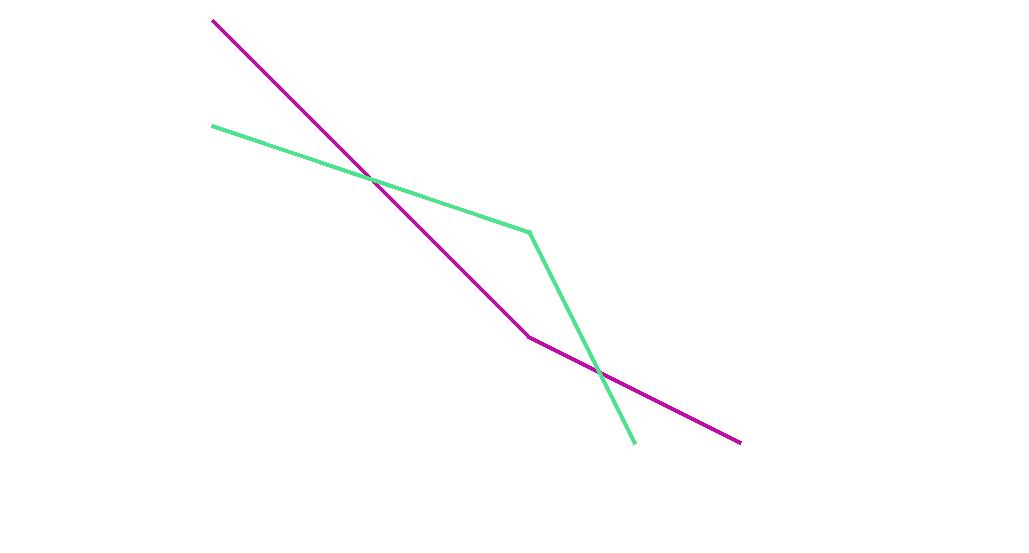
\includegraphics[width=0.65\linewidth]{3-4.png}}
% \end{figure*}
% 


% \section{User-interfaces}
% 
% 
% 
% 
% \framebox[4in][l]{\prompt \cmd{this is a command, short}}


% 
\index{test0.dat}



\vspace{-7\baselineskip}\footnotetext{You must download the program and the example data set, please see page \pageref{download}.}
\vspace{7\baselineskip}




First of all, we must open the program (see page \pageref{openprogram}), read the data set and define the values of the parameters, to be used in this analysis. For test0.dat we will use the following values:

\begin{center}
\begin{tabular}{ll}
\tui{c}ut & 0.25\\
\tui{r}ules & 0.75 0.5 1\\
\tui{m}inimal congruence & 0.8
\end{tabular}
\end{center}


\vspace{-7\baselineskip}\footnotetext{please remember:\\
to set each of these parameters you have to type the letters inside the square brackets [ ] and write the corresponding value followed by and [enter] or [return]}
\vspace{7\baselineskip}


\textbf{Search options}: Once the parameters have been defined, we will search for the general patterns of distribution. 

As we might have similar initial MSTs, we need to reduce them taking into account the similarity among the individual tracks to join
(gro\tui{u}p of tracks) and the value of \tui{m}inimal congruence fixed.
 
In the case of test0.dat, we gro\tui{u}p from the track number 1 [first] to the track number 6 [last]. Thus, we find whether there are similar individual tracks that can be consider as the same track, and those tracks will be joint. 


Later, we might need to redefine the values of the paramaters, in the case of test0.dat we will set:
\index{parameters:modify}


\begin{center}
\begin{tabular}{ll}
\tui{c}ut & 0.5\\
\tui{r}ules & 1.5 1 2\\
\tui{m}inimal congruence & 0.8
\end{tabular}
\end{center}



Then, Typing \tui{a}ll, we will find the congruent segments for each individual tracks in order to delimitate the generalized tracks or distributional patterns of species.

Finally, we need to eliminate those redundant generalized tracks, typing again \tui{u}, but joint from the track number 7  to the track 9, because first six tracks are individual tracks.

\textbf{Write a kml file}

Now, we need to write our results (the generalized tracks) in a kml file. To do that, first we must type \tui{k} and \tui{+} to activate the output to the  kml file. The kml info must change from FALSE to TRUE. Then, we will use \tui{w} if we want to write the whole information of the analysis including: individual tracks, and generalized tracks, or we can type \tui{e} to write only the generalized tracks into the kml file.
\vspace{-7\baselineskip}\footnotetext{.kml file extension is mandatory with googleearth, otherwise googleearth will complain and will not open the file}
\vspace{7\baselineskip}

\subsection{Command line interface}
\index{cli:command line interface}

For the command-line user interface we need to specified: 

the input file, 

the output file, 

and the parameters file.


For linux 64 bits:
\vspace{-7\baselineskip}\footnotetext{
CL typography: commands will be  \pname{croizat0}, to indicate that the instruction is named Croizat0 and you must type \pname{croizat0} in your parameter file, the command could be written using lower or upper case.}
\vspace{7\baselineskip}


\framebox[4.3in][l] {\prompt \cmd{ ./{\mt}-64 <input file> <output file> <parameters file>}}


%
%For linux 32 bits:
%
%\framebox[4.4in][l] {\prompt \cmd{ ./{\mt}-32 <input file> <output file> <parameters file>}}
%


For Windows 64 bits:

\framebox[4.4in][l] {\prompt \cmd{ {\mt}-64.exe <input file> <output file> <parameters file>}}


For Windows 64 bits:

\framebox[4.4in][l] {\prompt \cmd{ {\mt}-32.exe <input file> <output file> <parameters file>}}


\textbf{Output file:} it must have an extension .kml. 


\textbf{parameters file:} This interface was designed for parameters/searching strategies defined previously. These search strategies have to be set in the parameters file. There are two main predefined strategies, \pname{croizat0}, and \pname{croizat1}.




The framework of \pname{croizat0} is: 
\begin{enumerate}
 \item Find similar individual tracks [=\tui{u}] from the first, to the last individual track
 \item Calculate the congruent segments among individual tracks (delimitate generalized tracks) [= \tui{a}]
 \item Find similar generalized tracks  [=\tui{u}] from the first, to the last generalized tracks
\end{enumerate}
Therefore, our analysis made with the TUI is a \pname{croizat0} analysis.


The framework of \pname{croizat1} is: 
\begin{enumerate}
 \item Calculate the congruent segments among individual tracks (delimitate generalized tracks) by \tui{a}
 \item Find similar generalized tracks by \tui{u} from the first, to the last generalized tracks
\end{enumerate}

Thus, the commands for the analysis of test0.dat, using par1-search1.txt are:
\index{test0.dat: command line run}

For linux 64 bits:

\framebox[4.4in][l] {\prompt \cmd{ ./{\mt}-64 test0.dat test0.kml par1-search1.txt}}

% 
% For linux 32 bits:
% 
% \framebox[4.4in][l] {\prompt \cmd{ ./{\mt}-32 test0.dat test0.kml par1-search1.txt}}


For Windows 64 bits:

\framebox[4.5in][l] {\prompt \cmd{ {\mt}-64.exe test0.dat test0.kml par1-search1.txt}}

 
 For Windows 32 bits:
 
\framebox[4.5in][l] {\prompt \cmd{ {\mt}-32.exe test0.dat test0.kml par1-search1.txt}}
 


\subsection{Results of test0.dat analysis}


\begin{figure}[!ht]
\begin{center}
 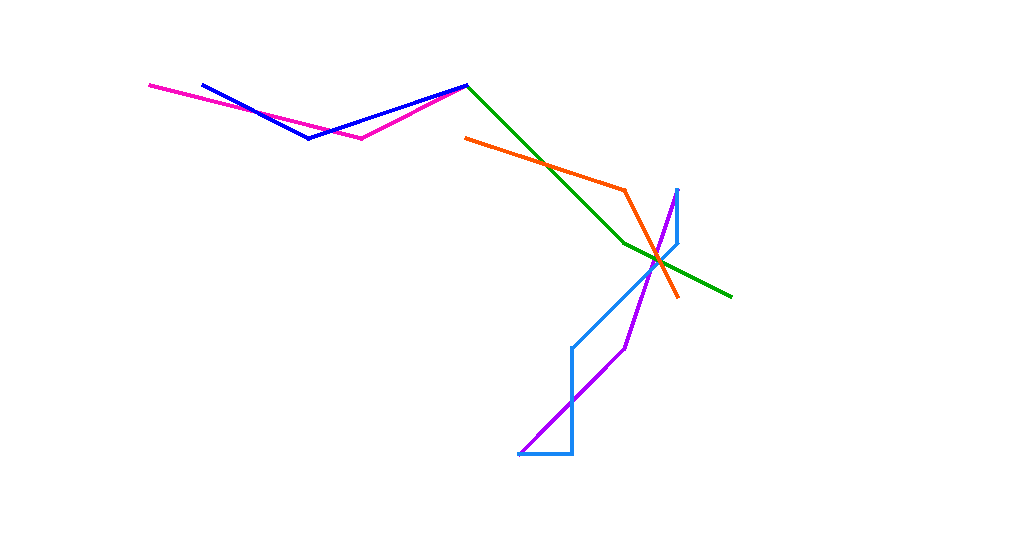
\includegraphics[scale=0.5]{./graphics/mst.png}
 % mst.png: 1029x553 pixel, 96dpi, 27.22x14.63 cm, bb=0 0 772 415
\end{center}
\caption{{\bf Individual tracks from test0.dat}}
\label{Figure1}
\end{figure}


\begin{figure}[!ht]
\begin{center}
 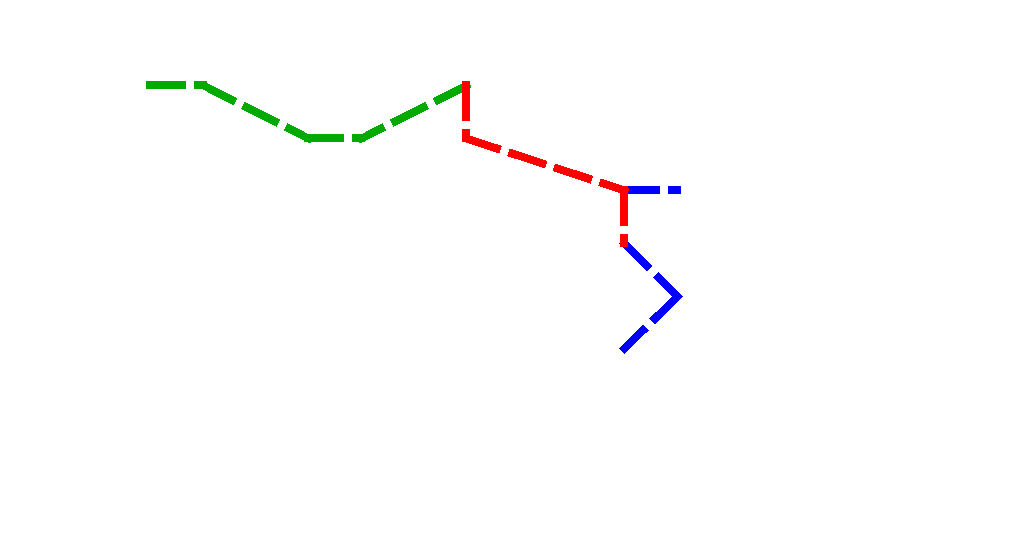
\includegraphics[scale=0.5]{./graphics/gtrack.png}
 % gtrack.png: 1029x553 pixel, 96dpi, 27.22x14.63 cm, bb=0 0 772 415
\end{center}
\caption{{\bf Generalized tracks from test0.dat}}
\label{Figure2}
\end{figure}





 

\chapter{PanTrack commands}


\label{ch:commands}
\index{commands}

\section{Text interface mode}
\label{tui_commands}
\index{commands:text interface}

	general
	
	\tui{l} == list			List all tracks
	
	
	comparing *tracks*
		
	\tui{a} == all			Track all the species using MSTs to compare			
	
	\tui{g} == group		Track a group of contiguous species
	
	\tui{p} == pair			Track a pair of species (contiguous or not)
	  
	In all the three cases a new MST=track will be created if the
	species compared are congruent, while in a [p]air comparison
	only a single track could be created. In an [a]ll/[g]roup 
	comparison, there could be more than one track.


	comparing *segments*
		
	\tui{s} == all			Track all the species using segments to compare			
		
	\tui{t} == pair			Track a pair of species (contiguous or not)
	  



	join

	
	\tui{u} == join group	Join a group of contiguous tracks if a given pair 

							has a minimal congruence equal or higher than the

							minimal congruence inputed in the value file or

							the default value used in the TUI. If you want to join

							a group regardless of the minimal congruence value,

							reduce the min. cong. value to 0.0. After this late

							analysis, replace the original min. cong. value
						

	\tui{j} == join pair		Join two, contiguous or not, tracks independent of

						the minimal congruence value
						

	congruence calculation
	
	\tui{o} == congr. group	Calculate the congruence by pairs of a contiguous group,

						as ther output is a list, is easier to reade a small 

						group than a large group
							

	\tui{n} == congr. pair	Calculate the congruence of a single pair 
	

	modify decision rules
	
	\tui{c} == cut			Change the minimal cut value

	\tui{r} == rules			Modify rules 

	\tui{m} == min. cong.		Change the minimal congruence value (see join)
	


\section{Bash command mode}
\label{bash_commands}
\index{commands:bash}

A bash command is an instruction that will perform an analysis equal to the analysis made in the text user interface [ see page \pageref{tui_commands}]. This mode is more appropriated to medium to huge data sets, where the analysis could last more than a few minutes or to test different parameter values. 

The commands are given in the equivalence of the TUI, with a short explanation.


		\cmd{kmlgen} == 	write to the kml file ONLY the generalized tracks (default). Must be in the file before the analysis. 

		\cmd{kmlall} == 	write to the kml file all, individual and generalized tracks. Must be in the file before the analysis.


		\cmd{croizat0} ==\\ 	join (individual tracks),\\ 
							track  (individual tracks),\\ 
							join (generalized tracks) \\
							%
= \tui{u} (1 - \# individual tracks), %
\tui{a},
\tui{u} ( individual tracks + 1) total tracks

		\cmd{croizat1} == \\	track  (individual tracks)\\ 
							join (generalized tracks)\\ 
= \tui{a}, \tui{u} (individual tracks +1) total tracks



A sample command file is 


\cmd{set cv 1.5}\\
\cmd{set lmax 2.0}\\
\cmd{set lmin 0.6}\\
\cmd{set maxline 3.0}\\
\cmd{set ci 0.80}\\
\cmd{kmlall}\\
\cmd{croizat0}\\

So, these seven lines in a file will change the default parameters to 
\cmd{cv = 1.5},
\cmd{lmax = 2.0},
\cmd{lmin = 0.6},
\cmd{maxline = 3.0},
\cmd{ci = 0.80},
and will use these values to join the indidual tracks if the congruence value of the two MSTs compared is larger than  0.80, then \MT  will track those resulting MST to obtain the generalized tracks and will eliminate (joint) those redundant tracks using the same rule used before (\cmd{ci = 0.80}), and will output the individual and the generalized tracks.   



%%
% The back matter contains appendices, bibliographies, indices, glossaries, etc.


\backmatter

\bibliography{manual}


\printindex

\end{document}

